\documentclass[UTF8]{ctexart}
\usepackage{float}
\usepackage{graphicx}
\begin{document}
\newpage
\section{概述}
\subsection{编写目的}
随着信息化进程的深入和数字设备市场的繁荣,全球产生的数据量正以大约每两年翻一番的速度增长。数据作为日渐重要的新型资产,其拥有者需要与之数据体量相匹配的存储能力来应对数据创造、采集、管理和存储的技术需求,巨大的设备和服务市场空间吸引着大批企业投身服务于整个数据生命周期的存储市场。
\begin{figure}[H]
  \centering
  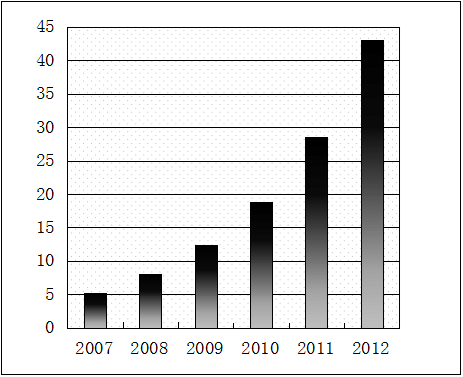
\includegraphics[width=0.9\textwidth]{part-one-1.png}
  \caption{IDC咨询报告中全球数据存户总量增长的图示}
\end{figure}
从上图可以看出,从2007年到2012年,全球数据总量以52\%的年复合增长率发展,尤其是基于文件数据的存储,每年的年复合增长率达到了69.4\%。如果采用传统的存储方式,那么需要的服务器,包括硬件、软件和网络等将不可估量,传统的网络存储已不能满足目前庞大的数据存储市场需求。
网络世界让世界触手可及,文件同步存储则是让跨越时空的不同客户、不同应用、不同屏幕实现无缝信息分享和服务互动体验的关键信息基础设施。面向文件同步存储市场的战略机遇,致力于从单纯电信服务向电信、信息和娱乐综合服务转型的电信运营商们纷纷构建自己的文件同步存储服务能力,并将其融入面向不同客户群的各类产品和解决方案中,基于宽带网络提供客户所需的文件共享、归档和备份等基础功能。
文件同步存储的出现,是存储行业技术和服务的一个重要创新和变革,它将解决众多用户对存储的低价、海量、安全、稳定要求。
釆用传统的本地存储策略己经逐渐难以满足人们对信息的存储和管理需要,而文件同步存储技术的提出,成为了一种解决信息数据存储和管理的有效途径,它不仅能够提供无限的空间,而且十分经济。分布式计算和网格计算的综合改进,是通过网络以按需、易扩展的方式获取所需服务的在线网格服务交付和使用模式,是分布式计算的一种方式,是网络上的服务以及提供这种服务的数据中心的软硬件集合。既然云计算基础设施之一是提供可靠、安全的数据存储中心,因此,存储安全是云计算中的重要话题之一。为了解决数据的保护问题,常见的方法是对用户数据进行加密。除了数据的私密性,其存储效率也非常重要。并且,当保存在云服务器端的密文数据发展到了一定的规模时,解决对数据的有效存储将是一个非常有意义的问题,我们也需要一个能够有着更高效率、损失更小的压缩算法来对网络中的数据进行压缩,尽管可能在本地解压的时间成本会耗费一些,但是相比起大量数据的传输代价,这点代价已经非常能够被人接受。

\subsection{项目背景}
当前有很多在线文件存储系统,如DropBox、subversion、百度网盘等,能够将存储在本地的文件自动同步到云端服务器保存。因为云端服务的特性,存储成本可以被无限摊薄。

Dropbox优点是易用和对用户零干扰。当两个用户同时对一个文件进行编辑,后提交会多生成冲突文件,留给用户线下来解决,不会象SVN 一样提醒用户。安全从两个方面看,一是可靠性,dropbox会将本地数据当作一个副本,当服务器端数据没了,会自动上传,另外声称在AWS上保存有数据,对数据可靠性较高,如果丟失基本上是元数据损坏,从设计看是以用户隔离的。

百度网盘的优点是操作简单,免费容量较大,使用范围广,互动性强。

尽管现在有多种在线文件存储系统,然而网络传输、用户保障等问题依然存在。

\subsection{国内外发展现状}
用户渴望能够充分利用IT资源来给业务提供及时按需的高效服务。云存储是在云计算概念上延伸和发展出来的一个新的概念,在云计算发展的轨迹中,随处都可以看到存储云化发展的身影。
在技术方面,现代存储技术从磁带发展到磁盘、再从磁盘发展到阵列、继而从阵列发展到网络存储,而今,又随着集群技术、网格技术、分布式存储技术、虚拟化存储技术的发展,进入了文件同步存储的时代。

文件同步存储是近年来发展起来的一个一个新兴技术,各大企业都将精力投入到了文件同步存储的研究中。随着云计算技术受到广泛的关注,文件同步存储技术也得到了广泛的重视。文件同步存储可以在一系列软件的支撑下将多种存储设备进行整合,构成海量存储空间空用户使用。利用文件同步存储服务,可以大大节省存储空间,并且节约成本。文件同步存储技术是云计算技术的延伸,该技术通过使用多种技术手段如集群应用、网格技术、分布式文件系统等,将多种存储设备进行整合,实现不同架构存储设备的协同工作,供用户进行数据存储和业务访问等,也可以使用良好的压缩算法来岁。

国内文件同步存储公众应用虽起步比国外晚,但目前也已经涌现了多个成功应用。比较著名的有华为网盘、115网盘、金山快盘和新浪微盘等。华为网盘的优势在于其针对中、高端用户的套餐内容较多,覆盖面比较广,支持的单次上传文件较大(最大可至24GB)。115网盘主要的客户群是中小客户,其稳定性较好,共享方式较灵活,社交功能非常强大。金山快盘的优势在于其同步备份文件的速度较快,跨平台同步的无缝衔接性较好,云端相册浏览体验犹如行云流水。而新浪微盘依托着新浪微博的强大人气应运而生,依托新浪微博为媒介的共享功能是其最大亮点,其“热门分享”有效吸引了用户分享文件的积极性。

尽管国内外的文件同步存储应用已经很多,但是对于压缩算法的使用上有以下一些比较典型的:香农编码用树形结构编译模型数据,顺序是从根到叶,产生编码长度可变的码词。估计码词长度的准则是符号出现的概率。符号出现的概率越大,其码词的长度越短。如今的音频文件和图片文件中用到的Huffman算法是通过从叶到根的顺序,与香农编码不同的在于不需要另外附加同步代码,因此有着更佳的表现。LZW算法是从一端到另一端的数据流模式,比较适用于重复率很高的文本压缩。Misra的算法,是从数据的中间部分向外压缩,同时逆向查找数据中的隐藏结构并压缩。

\subsection{项目必要性及意义}
虽然当前已有很多优秀的在线文件存储系统,但是它们仍然存在一些问题。比如Dropbox在国内使用不了,而百度云使用协议中, “我们也保留随时单方决定中止或结束服务的权利,恕不另行通知。例如,如果您未遵守这些条款,或者您使用服务的方式将使我们承担法律责任、干扰服务运行或干扰他人使用服务,我们可以中止或终止您使用我们的服务”,也就是使用无保障。

我们提出了一种名为QuarkBox的全新在线文件存储系统,它除了实现在线文件存储系统的基本功能之外,更针对以上现存文件系统的不足之处进行改进。此外,QuarkBox利用高效无损压缩算法Quarkzip对文件进行无损压缩,大大提升了网络传输效率和使用体验。对于此类系统而言,本地的解压代价相对传输是很小的。因为我们的Quarkzip算法可以把任意文件进行无损压缩,那么它在网络环境中传输就有很大优势。

概括来说,QuarkBox项目有以下必要性和意义:

\begin{itemize}
\item 高效实现DropBox的所有功能
  \begin{itemize}
  \item (本地)快速无损压缩
  \item (云端)预览时解压缩、预览时解压缩
  \item 文件分享,上传,公共API开放
  \item 文件多版本(历史版本)管理
  \item 图片文件自动除重选择最优功能
  \item 增量同步
  \end{itemize}
\item Quarkzip高效无损压缩,提高网络传输性能
\item 同时提供国内外支持
\item 对比百度云等,提升了用户使用保障
\end{itemize}

\end{document}
